\documentclass{article}
\usepackage{iclr2026_conference,times}
\input{math_commands.tex}
\usepackage{amsmath,amssymb,amsthm}
\usepackage{booktabs}
\usepackage{graphicx}
\usepackage{hyperref}
\usepackage{microtype}
\usepackage{url}
\newcommand{\ResultPreset}{smoke}
\newcommand{\MainStaleFraction}{0.85}
\newcommand{\MaxN}{64}
\newcommand{\NaiveNOneTrue}{-5.30}
\newcommand{\NaiveMaxTrue}{-13.29}
\newcommand{\NaiveMaxProxy}{-2.40}
\newcommand{\NaiveMaxGap}{10.88}
\newcommand{\NaiveMaxHallucination}{27.8\%}
\newcommand{\NaiveMaxPrecision}{13.7\%}
\newcommand{\NaiveMaxStale}{86.3\%}
\newcommand{\BaseMaxTrue}{-0.19}
\newcommand{\RepairedMaxTrue}{-1.95}
\newcommand{\RepairedMaxHallucination}{0.0\%}
\newcommand{\RepairedMaxPrecision}{47.7\%}
\newcommand{\RepairedMaxStale}{52.3\%}
\newcommand{\OracleMaxTrue}{-1.55}
\newcommand{\RepairGain}{11.33}
\newcommand{\OracleGap}{0.40}


\title{When More Rollouts Remember the Wrong Thing:\\Best-of-N Amplifies Stale Memory in Retrieval-Augmented World Models}

% The ICLR submission style keeps this anonymous while \iclrfinalcopy is commented.
\author{Anonymous Authors}

%\iclrfinalcopy

\newtheorem{proposition}{Proposition}
\newcommand{\bon}{Best-of-N}
\newcommand{\meg}{\mathrm{MEG}}

\begin{document}
\maketitle

\begin{abstract}
Memory-augmented world models retrieve episodic transitions, trajectories, or cases
to improve prediction under sparse data. Separately, \bon{} inference samples many
candidate futures and selects the one with the highest model proxy. This paper
studies a narrow interaction between the two: stale or support-mismatched memory
can create rare \emph{memory-impostor} rollouts with high predicted value and low
true value, and \bon{} makes those rollouts more likely to be selected. We give a
finite-N mechanism statement, propose diagnostics based on retrieval precision,
staleness, counterfactual memory dropout, and proxy-true gap, and instantiate the
mechanism in a controlled latent-regime world. In the main stale-memory condition,
naive memory \bon{} improves its proxy score while true return falls from
\NaiveNOneTrue{} at $N=1$ to \NaiveMaxTrue{} at $N=\MaxN{}$; selected rollouts
have \NaiveMaxPrecision{} retrieval precision, \NaiveMaxStale{} stale retrieval,
and \NaiveMaxHallucination{} hallucinated-rollout rate. A repair using recency
retrieval, disagreement-aware memory gating, and dropout-risk penalties reaches
\RepairedMaxTrue{} true return at the same $N$, narrowing but not eliminating the
gap to an oracle retriever. The claim is intentionally scoped: this is a runnable
diagnostic for an architecture-specific failure mode, not evidence that memory is
generally harmful.
\end{abstract}

\section{Introduction}

World models let agents reason in imagined futures rather than only through
environment interaction \citep{sutton1990dyna,ha2018worldmodels,hafner2019planet,hafner2020dreamer,schrittwieser2020muzero}. A
common inference pattern is to sample many candidate rollouts and select the one
with the highest model score. This is attractive whenever the generator is cheap
and the scoring proxy is believed to be reliable.

External memory gives a second source of test-time power. Episodic control,
retrieval-augmented reinforcement learning, case-based reasoning, kNN language
models, and retrieval-augmented generation all show that non-parametric memory
can improve adaptation and factuality
\citep{aamodt1994cbr,pritzel2017nec,wayne2018merlin,khandelwal2020knnlm,guu2020realm,lewis2020rag,goyal2022rarl}. For world
models, the hope is direct: retrieve relevant cases and make better local
transition predictions.

This paper asks what happens when these two useful ideas are composed under
support mismatch. If the retriever returns stale cases from a latent regime with
the wrong transition sign, a memory-augmented model can assign high value to a
candidate future that the real environment will not realize. \bon{} then searches
for that error. More samples need not make the selected rollout more grounded;
they can make it a better impostor under the memory-biased proxy.

Our contributions are:
\begin{itemize}
    \item a finite-N statement of memory-impostor amplification;
    \item diagnostics for selected-rollout retrieval precision, staleness,
    memory dropout variance, hallucinated-rollout rate, and the memory
    exploitation gap;
    \item a controlled synthetic world where latent dynamics, memory provenance,
    and true rollout utility are all known;
    \item a simple repair that combines recency-aware retrieval,
    disagreement-aware memory gating, and an uncertainty penalty.
\end{itemize}

\section{Related Work}

\textbf{World models and model-based RL.}
Model-based RL has long used learned dynamics for planning
\citep{sutton1990dyna}. Modern world models learn latent dynamics from high-dimensional observations and use imagined trajectories for control
\citep{ha2018worldmodels,hafner2019planet,hafner2020dreamer}. Probabilistic and
offline model-based methods such as PETS, MBPO, MOReL, and MOPO explicitly
address model bias and uncertainty \citep{chua2018pets,janner2019mbpo,kidambi2020morel,yu2020mopo}. Our setting is not a new
planner; it isolates a failure source that arises when the local dynamics model
is partly retrieved from an external case memory.

\textbf{Episodic, retrieval, and case-based memory.}
Case-based reasoning formalized retrieve/reuse/revise/retain cycles
\citep{aamodt1994cbr}. Neural episodic control and MERLIN showed that fast
memory can help agents adapt \citep{pritzel2017nec,wayne2018merlin}, while
retrieval-augmented RL and model-based episodic memory bring retrieved
experience into control and model-based settings
\citep{goyal2022rarl,le2021mbem}. Retrieval-augmented language models and
kNN-LMs show a closely related non-parametric interpolation pattern
\citep{khandelwal2020knnlm,guu2020realm,lewis2020rag,borgeaud2022retro,wu2022memorizing}.
These works motivate memory augmentation; our contribution is to show how
inference-time selection can amplify a memory error that average prediction
metrics may understate.

\textbf{Test-time selection and proxy optimization.}
Self-consistency, verifier ranking, Tree of Thoughts, and test-time compute
scaling all improve outputs by sampling or searching multiple candidates
\citep{wang2023selfconsistency,cobbe2021verifiers,yao2023tree,snell2024testtime}.
Reward-model overoptimization shows that selecting against an imperfect proxy can
degrade true utility \citep{gao2023reward}. Our finite-N argument is simple in
that tradition; the novelty is the memory-specific source of proxy/true
inversion and the corresponding retrieval diagnostics.

\section{Mechanism}

Let a candidate rollout be grounded with probability $1-p$ and a
memory-impostor with probability $p>0$. A memory-impostor is a rollout whose
model score is high because retrieved cases are stale or support mismatched, but
whose true return is low under the environment dynamics. Suppose every impostor
has proxy score $s_I$ and true utility $u_I$, and every grounded candidate has
proxy score $s_G$ and true utility $u_G$, with $s_I>s_G$ but $u_I<u_G$.

\begin{proposition}[Finite-N memory-impostor amplification]
If a \bon{} selector chooses the candidate with highest proxy score from $N$
independent samples under the two-type model above, then
\[
P(\text{impostor selected}) = 1-(1-p)^N,
\]
and the expected true utility of the selected candidate is
\[
\mathbb{E}[u_N] = \left(1-(1-p)^N\right)u_I + (1-p)^N u_G,
\]
which decreases monotonically in $N$.
\end{proposition}

The proposition is not presented as deep probability theory. Its purpose is to
turn a reviewer's likely objection into a diagnostic: if memory retrieval can
produce high-proxy low-true candidates, increasing $N$ should increase proxy
score, selected memory staleness, and proxy-true gap while decreasing true
return.

\section{Diagnostic and Repair}

For a selected rollout $\tau$, define the memory exploitation gap
\[
\meg(\tau) = S_\text{model}(\tau)-U_\text{true}(\tau),
\]
where $S_\text{model}$ is the model proxy used for selection and $U_\text{true}$
is the environment return used only for evaluation. We also log retrieval
precision, stale retrieval rate, disagreement among retrieved transition signs,
and counterfactual memory dropout variance: the variance of predicted deltas
under leave-one-retrieved-case-out perturbations.

The repair intentionally uses only observable memory metadata and transition
statistics, not the hidden regime label. It has three parts. First, retrieval is
recency-aware, so recent calibration transitions can compete with dense stale
cases. Second, memory interpolation is gated down when retrieved cases disagree
or are old. Third, the \bon{} proxy is penalized by the average dropout-risk
score. This is a small repair rather than a claim of optimality; the point is to
test whether the diagnosis points toward an effective intervention.

\section{Controlled Benchmark}

The benchmark is a one-dimensional latent-regime world. The observed state is
position $x$ and actions are $a\in\{-1,0,1\}$. The current hidden regime is
\emph{reverse}, so the true transition is $x_{t+1}=x_t-a_t$. The memory store is
dense with stale \emph{forward} transitions where $x_{t+1}=x_t+a_t$ and sparse
with recent reverse calibration transitions. A naive nearest-neighbor retriever
sees only $(x,a)$, so the stale forward cases often dominate.

Candidate action sequences are sampled with both directional modes. Each model
rolls out every candidate, scores the predicted final distance to a fixed goal,
and executes the proxy-best sequence under the true reverse dynamics. We compare
four selectors: a non-memory model fit from recent calibration transitions,
naive memory, oracle memory that is allowed to filter by the hidden regime, and
the repaired memory model.

\section{Results}

\begin{figure}[t]
    \centering
    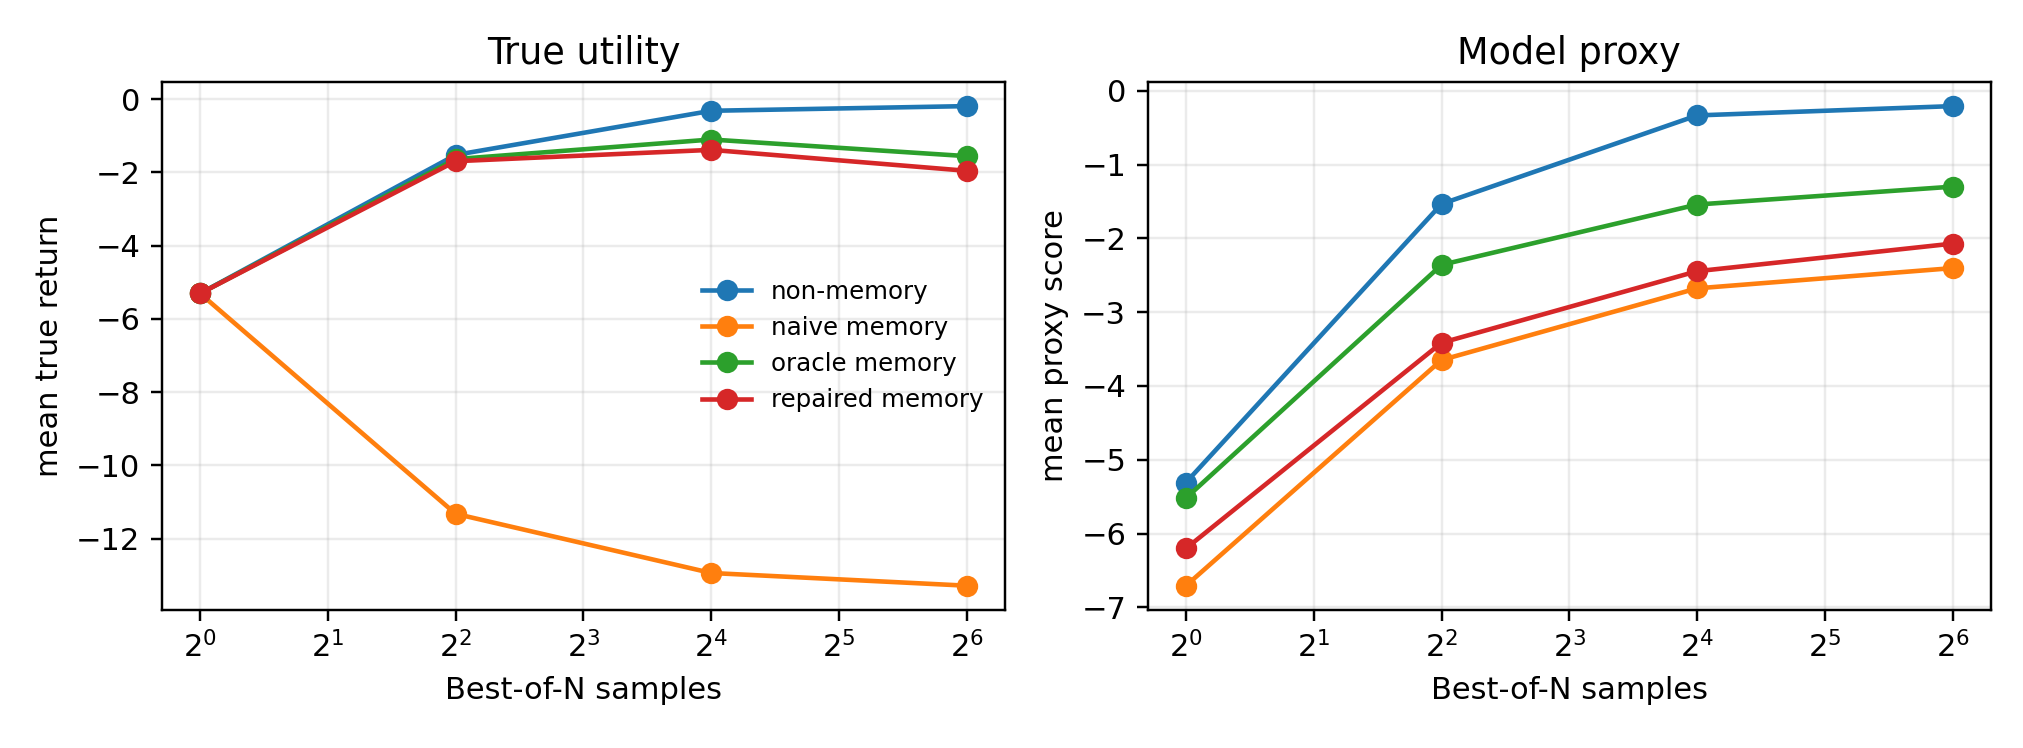
\includegraphics[width=\linewidth]{figures/bon_scaling_curves.png}
    \caption{In the stale-memory condition, naive memory \bon{} improves model
    proxy score as $N$ grows while true return degrades. The repaired selector
    tracks the non-memory/oracle direction because it suppresses stale retrieved
    transitions.}
    \label{fig:scaling}
\end{figure}

Figure~\ref{fig:scaling} shows the main scaling pattern. At stale fraction
\MainStaleFraction{}, naive memory \bon{} falls from \NaiveNOneTrue{} true return
at $N=1$ to \NaiveMaxTrue{} at $N=\MaxN{}$, even though its selected proxy score
is \NaiveMaxProxy{}. The resulting exploitation gap is \NaiveMaxGap{}. The
non-memory baseline reaches \BaseMaxTrue{}, the repaired model reaches
\RepairedMaxTrue{}, and the oracle retriever reaches \OracleMaxTrue{}.

\begin{figure}[t]
    \centering
    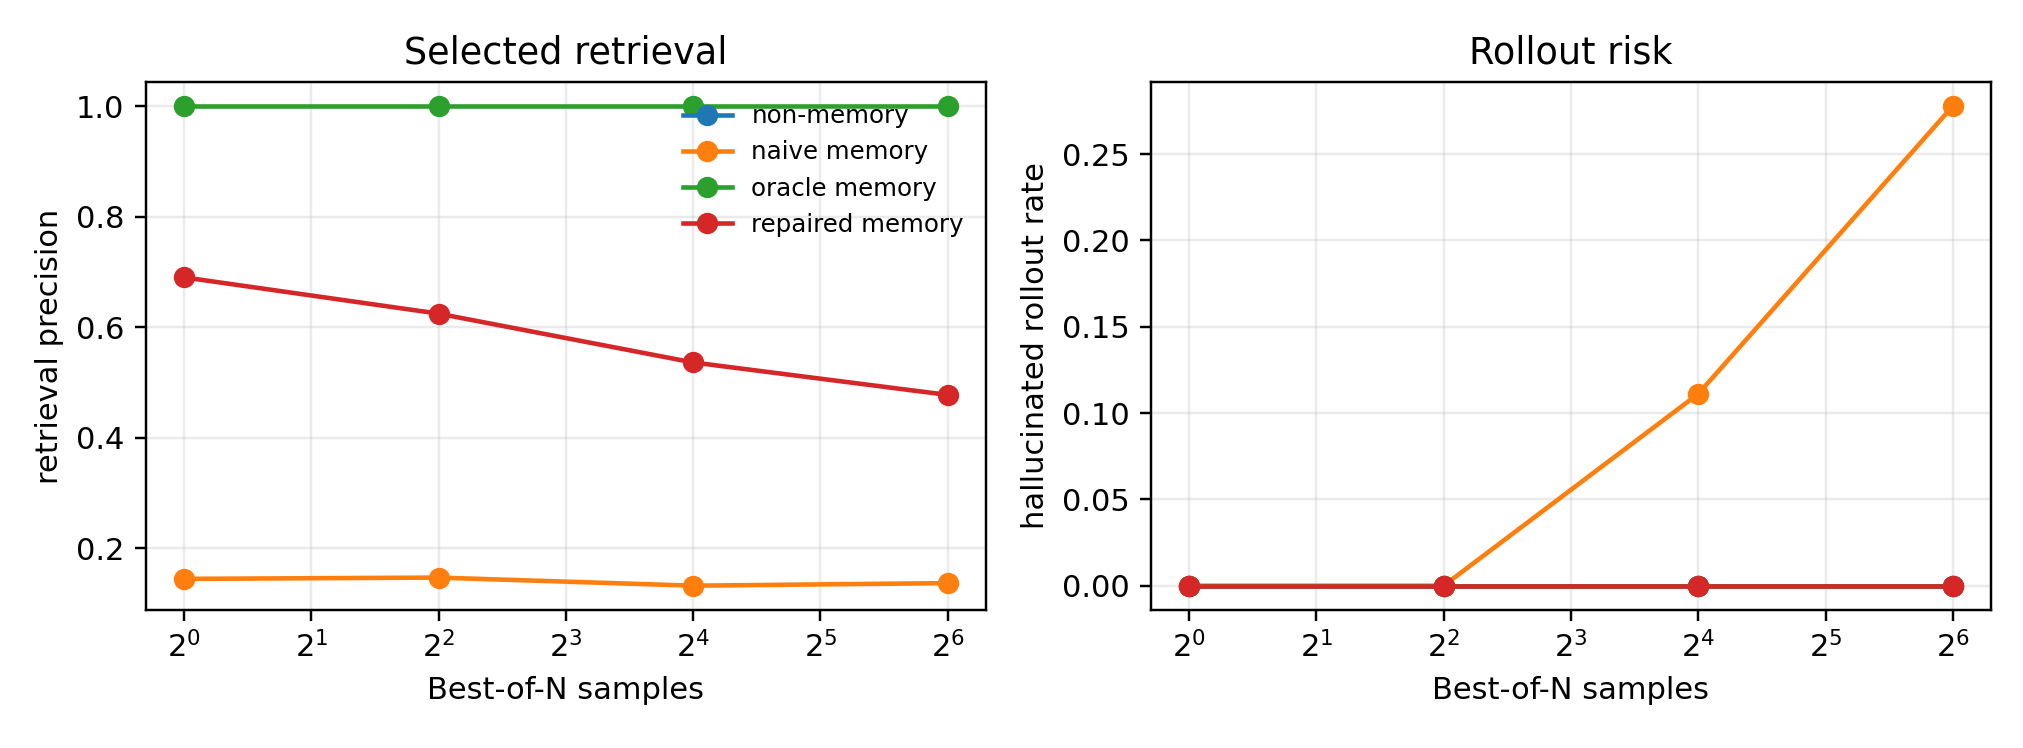
\includegraphics[width=\linewidth]{figures/retrieval_diagnostics.png}
    \caption{Selected-rollout diagnostics reveal the mechanism. Naive memory
    selections have poor retrieval precision and a high hallucinated-rollout
    rate at large $N$; the repair improves selected retrieval quality and
    sharply reduces hallucinated rollouts.}
    \label{fig:diagnostics}
\end{figure}

Figure~\ref{fig:diagnostics} confirms that the failure is not merely bad random
actions. At $N=\MaxN{}$, naive selected rollouts have \NaiveMaxPrecision{}
retrieval precision and \NaiveMaxStale{} stale retrieval. Their hallucinated
rollout rate is \NaiveMaxHallucination{}. The repaired model improves selected
retrieval precision to \RepairedMaxPrecision{}, lowers stale retrieval to
\RepairedMaxStale{}, and reduces hallucinated rollouts to
\RepairedMaxHallucination{}.

\begin{figure}[t]
    \centering
    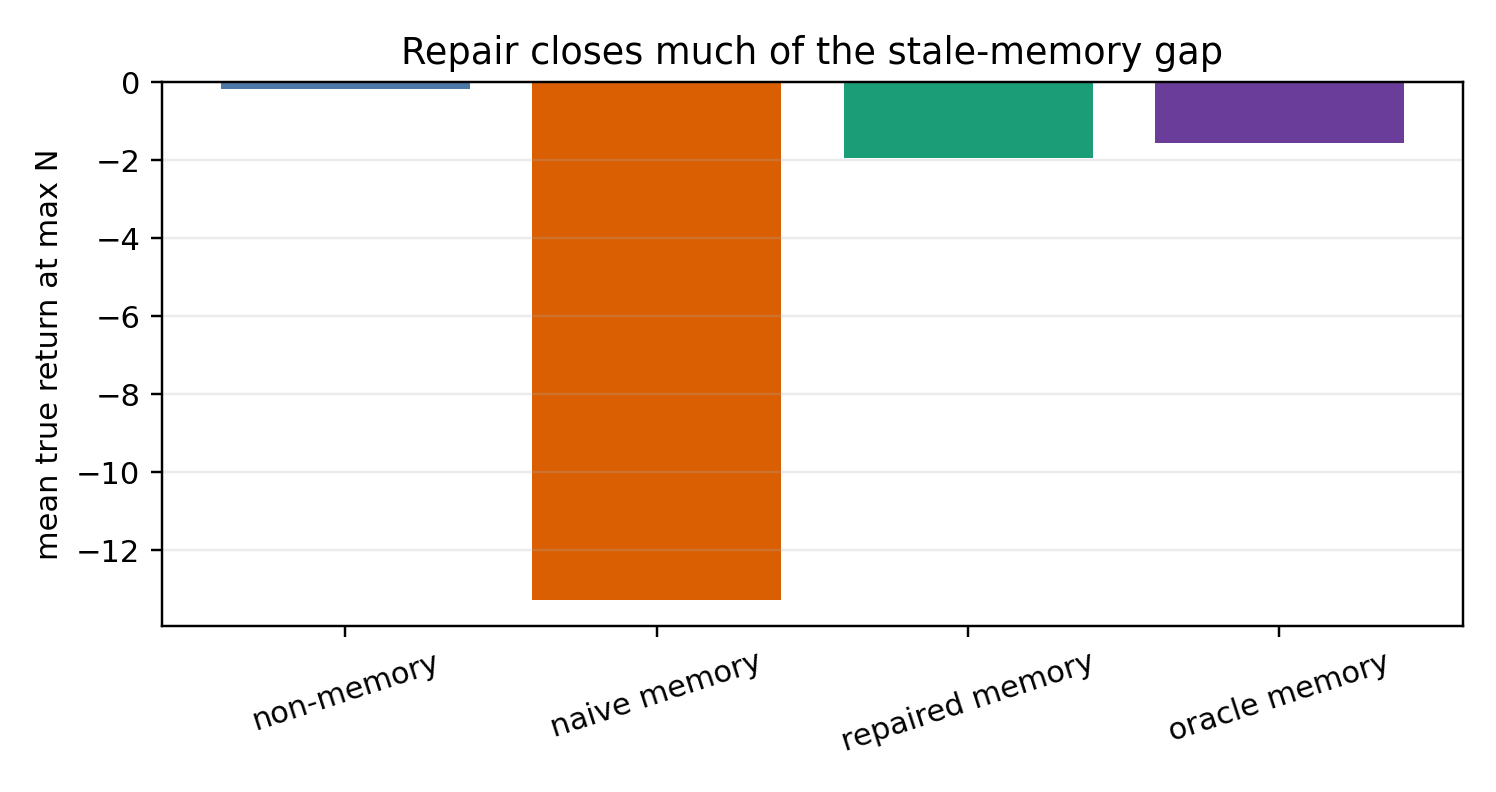
\includegraphics[width=0.78\linewidth]{figures/repair_gap.png}
    \caption{At the largest $N$, the repair improves true return by
    \RepairGain{} over naive memory. The remaining oracle gap is \OracleGap{},
    which is expected because the oracle can directly filter by hidden regime.}
    \label{fig:repair}
\end{figure}

Figure~\ref{fig:repair} makes the repair boundary visible. The repaired model is
not an oracle and does not claim to recover the hidden regime perfectly. It uses
age, disagreement, and memory-dropout risk as support diagnostics, which are
available to a memory system without revealing the environment's latent label.

\section{Limitations}

The benchmark is synthetic and deliberately low-dimensional. That is a strength
for mechanism isolation and a weakness for external validity. The repair is also
minimal: realistic systems would need stronger retrieval calibration, diversity
constraints, causal or regime-aware memories, and task-specific uncertainty
models. Finally, the formal claim is only the two-type finite-N amplification
law; it does not prove that a particular neural retriever will produce impostors
in deployment.

\section{Reproducibility and Checklist}

The repository includes the full synthetic generator, tests, raw result CSVs,
plotting scripts, the 100+ entry related-work matrix, and this anonymous ICLR
source. The oracle baseline is explicitly marked as using the hidden latent
regime, while the repair is marked as non-oracle. No human-subject data or
private datasets are used. Compute is a CPU-only synthetic run.

\bibliographystyle{iclr2026_conference}
\bibliography{references}

\appendix
\section{Additional Diagnostic Definition}

The hallucinated-rollout indicator is one when the selected candidate's model
proxy is near-goal while its true return is poor. In code, this corresponds to a
proxy score above $-1.75$ and true return below $-5.0$. The threshold is used only
for diagnostics; selection itself uses the raw proxy or repaired proxy.

\section{Anonymous Submission Note}

The source uses \texttt{iclr2026\_conference.sty} and keeps
\texttt{\textbackslash iclrfinalcopy} commented. The resulting PDF displays the
standard under-review anonymous author block.

\end{document}
